%From https://egu2018.eu/PICO_how-to_guide_to_PICO.pdf
%Abstracted and templated by Brian Ballsun-Stanton, Macquarie University.
%original template by https://github.com/snowtechblog/pico-latex-presentation by Anselm Köhler

\documentclass[unknownkeysallowed,usepdftitle=false,aspectratio=169, parskip=full]{beamer}
% unknownkeysallowed is needed for mac and the newer latex version -> is more picky than before...
\usetheme[headheight=1cm,footheight=2cm]{boxes}
%\usetheme{default}


\usepackage{default}
\usepackage{graphicx}
%example pictures created via: http://lorempixel.com/1200/800/cats/Figure2/. Credit to http://lorempixel.com/images.php

\usepackage{epsfig}
\usepackage{siunitx}
\usepackage{color}
\usepackage{ifthen}
\usepackage[rightcaption]{sidecap}
\usepackage[font=scriptsize,labelfont=bf]{caption}
%usepackage{ragged2e}

\usepackage[T1]{fontenc}
\usepackage[utf8]{inputenc}
%https://tex.stackexchange.com/a/203804/5483

\usepackage[activate={true,nocompatibility},final,tracking=true,kerning=true,spacing=true,factor=1100,stretch=10,shrink=10]{microtype} % http://www.khirevich.com/latex/microtype/
\microtypecontext{spacing=nonfrench}

\usepackage{lipsum} % for dummy text only
\usepackage[UKenglish]{babel} %https://tex.stackexchange.com/a/27743 
\usepackage[pangram]{blindtext} % https://tex.stackexchange.com/a/48411

%\usepackage{parskip} % from https://tex.stackexchange.com/q/11622
%\setlength{\parskip}{12pt} 

%\setparsizes{\parindent}{12pt}{\parfillskip}

%\usepackage{etoolbox} % as per https://tex.stackexchange.com/a/24331
%\appto\chapterheadendvskip{\vspace{-1\parskip}}
%\setparsizes{\parindent}{50pt plus 20pt minus 30pt}{\parfillskip}

\setbeamertemplate{navigation symbols}{}%remove navigation symbols
\setbeamersize{text margin left=1cm,text margin right=1cm}

% some colors
\definecolor{grau}{gray}{.5}
\definecolor{slfcolor}{rgb}{0,0.6274,0.8353}
\definecolor{wslcolor}{rgb}{0,0.4,0.4}

% setup links
\hypersetup{%
	%linkbordercolor=green,%
	colorlinks=false,%
	pdfborderstyle={/S/U/W 0},%
	%pdfpagemode=FullScreen,%
	pdfstartpage=4%
	}

% setup some fonts
\setbeamerfont{title}{series=\bfseries, size=\small}
\setbeamerfont{author}{size*={5pt}{0pt}}
\setbeamerfont{institute}{size*={3pt}{0pt}}
\setbeamerfont{bodytext}{size=\scriptsize}
	
% Title setup	
\title{Corpus Word Frequency Analysis}
\author{Jan Jugueta (\texttt{jan.jugueta@hdr.mq.edu.au})}
\institute{Macquarie University, North Ryde, NSW}
% add title in headbox
\setbeamertemplate{headline}
{\leavevmode
\begin{beamercolorbox}[width=1\paperwidth]{head title}
  % LOGO
  \vspace{0.1cm}
  \begin{columns}[t, totalwidth=\textwidth]
  \begin{column}[c]{1.05cm}
  \end{column}
  % TITLE
   \begin{column}[c]{10.6cm}
   \centering \usebeamerfont{title} \textcolor{slfcolor}{\inserttitle} \\
   \centering \usebeamerfont{author} \color[rgb]{0,0,0} \insertauthor \\
   \vspace{-0.05cm}
   \centering \usebeamerfont{institute} \insertinstitute
  \end{column}
  % PICTURE
  \begin{column}[c]{1.15cm}
    \hspace{0.005cm}
  \end{column}
  \end{columns}
  {\color{slfcolor}\hrule height 1pt\vspace{0.1cm}}
\end{beamercolorbox}%
}

% setup the navigation in footbox
% first set some button colors
\newcommand{\buttonactive}{\setbeamercolor{button}{bg=wslcolor,fg=white}}
\newcommand{\buttonpassive}{\setbeamercolor{button}{bg=slfcolor,fg=black}}
% now set up that the one active one gets the new color.
\newcommand{\secvariable}{nothing}
% therefore we write before each section (well, everything which should be part of the navi bar)
% the variable \secvariable to any name which is in the next function ...
\newcommand{\mysection}[1]{\renewcommand{\secvariable}{#1}
}
% ... compaired to strings in the following navibar definition ...
\newcommand{\tocbuttoncolor}[1]{%
 \ifthenelse{\equal{\secvariable}{#1}}{%
    \buttonactive}{%
    \buttonpassive}
 }
% ... here we start to set up the navibar. each entry is calling first the function \tocbuttoncolor with the argument which should be tested for beeing active. if active, then change color. afterwards the button is draw. so to change that, you need to change the argument in \toc..color, the first in \hyperlink and before each frames definition... A bit messed up, but works...
\newlength{\buttonspacingfootline}
\setlength{\buttonspacingfootline}{-0.2cm}
\setbeamertemplate{footline}
{\leavevmode
\begin{beamercolorbox}[width=1\paperwidth]{head title}
  {\color{slfcolor}\hrule height 1pt}
  \vspace{0.05cm}
  % set up the buttons in an mbox
  \centering \mbox{
    \tocbuttoncolor{abstract}
    \hyperlink{abstract}{\beamerbutton{2 Minute Madness}}
    \tocbuttoncolor{radar}
    \hspace{\buttonspacingfootline}
      \hyperlink{radar}{\beamerbutton{Workflow}}
     \tocbuttoncolor{slab}
    \hspace{\buttonspacingfootline}
      \hyperlink{slab}{\beamerbutton{Article to Text}}
    \tocbuttoncolor{line}
    \hspace{\buttonspacingfootline}
      \hyperlink{line}{\beamerbutton{Bash}}
    \tocbuttoncolor{major}
    \hspace{\buttonspacingfootline}
      \hyperlink{major}{\beamerbutton{R}}
   
    \tocbuttoncolor{minor}
    \hspace{\buttonspacingfootline}
      \hyperlink{minor}{\beamerbutton{Results}}
    \tocbuttoncolor{conclusion}
    \hspace{\buttonspacingfootline}
      \hyperlink{conclusion}{\beamerbutton{Conclusion}}
    % this last one should normaly not be used... it will open the preferences to change the 
    % behaviour of the acrobat reader in fullscreen -> usefull in pico...
    \setbeamercolor{button}{bg=white,fg=black}
    % for presentation
    %\hspace{-0.1cm}\Acrobatmenu{FullScreenPrefs}{\beamerbutton{\#}}
    % for upload
    
     
\Acrobatmenu{FullScreenPrefs}{\vspace{0.3cm}\hspace{0.24cm}\mbox{%
      \includegraphics[height=0.04\textheight,keepaspectratio]{%
	  figure/CreativeCommons_Attribution_License.eps}%
	  }}
   }
    \vspace{0.05cm}
\end{beamercolorbox}%
}


\begin{document}


%%%%%%%%%%%%%%%%%%%%%%%%%%%%%%%%%%%%%%%%%%%%%%%%%%%%%%%%%%%%%%%%%%%%%%%%%%
\mysection{abstract}
%%%%%%%%%%%%%%%%%%%%%%%%%%%%%%%%%%%%%%%%%%%%%%%%%%%%%%%%%%%%%%%%%%%%%%%%%%
\begin{frame}\label{\secvariable}
\begin{center}
\begin{figure}[h]
\centering
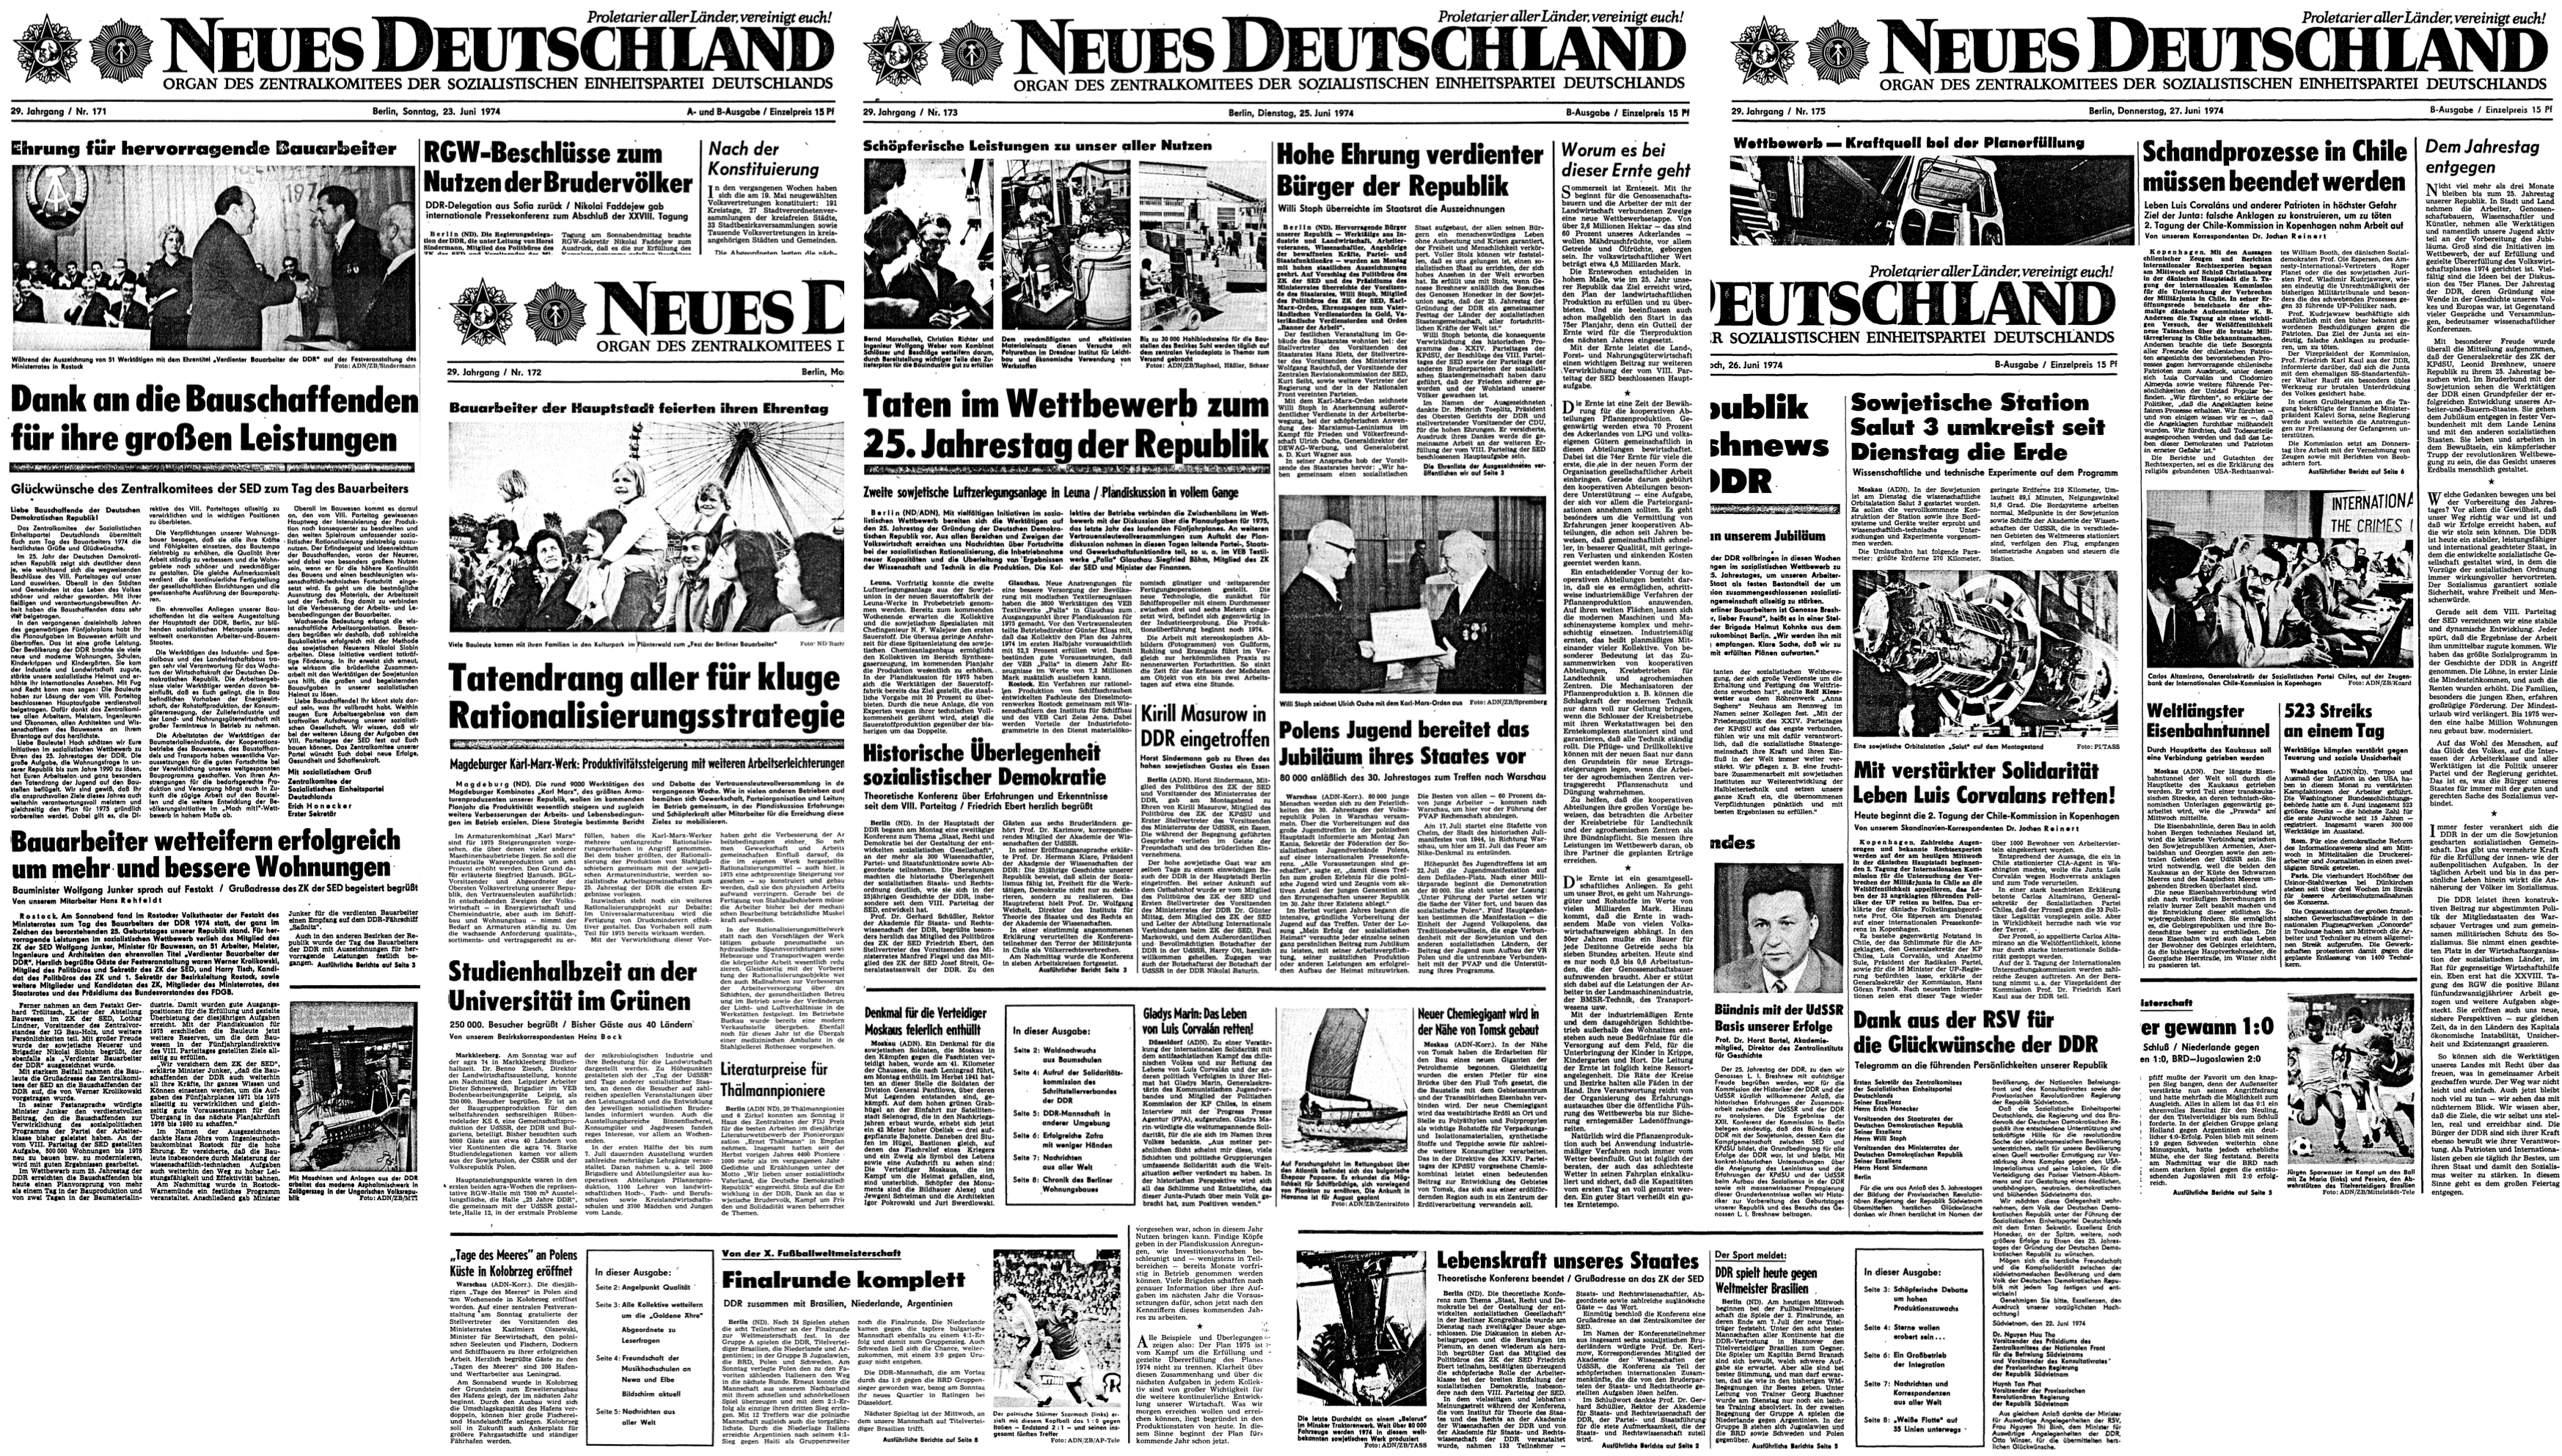
\includegraphics[width=0.8\textwidth,height=0.8\textheight,keepaspectratio]{figure/nd.png}
\caption{Five front pages from \textit{Neues Deutschland}. Adapted from Neues Deutschland, by Jan Jugueta, 2019, retrieved from http://nd-archiv.de/. Copyright 1974 by Neues Deutschland.}
\end{figure}
\end{center}
\end{frame}

\begin{frame}\label{\secvariable}
  \begin{columns}[t]
  %https://tex.stackexchange.com/a/7452/5483
  \begin{column}[c]{0.45\textwidth}
\begin{figure}[h]
\centering
\includegraphics[width=1\textwidth,height=1\textheight,keepaspectratio]{figure/corpus.png}
\caption{A corpus of \textit{Neues Deutschland} articles in .txt format. Adapted from Neues Deutschland, by Jan Jugueta, 2019, retrieved from http://nd-archiv.de/. Copyright 1974 by Neues Deutschland.}
\end{figure}
    \end{column}
    \begin{column}[c]{0.45\textwidth}
    \begin{figure}[h]
\centering
\includegraphics[width=0.8\textwidth,height=0.8\textheight,keepaspectratio]{figure/results.png}
\caption{Results from Body, Title and Title + Subtitle word frequency analysis. 
Screenshot by Jan Jugueta.}
\end{figure}
    \end{column}
    
  \end{columns}

  
\end{frame}

%%%%%%%%%%%%%%%%%%%%%%%%%%%%%%%%%%%%%%%%%%%%%%%%%%%%%%%%%%%%%%%%%%%%%%%%%%
\mysection{radar}
%%%%%%%%%%%%%%%%%%%%%%%%%%%%%%%%%%%%%%%%%%%%%%%%%%%%%%%%%%%%%%%%%%%%%%%%%%
\begin{frame}\label{\secvariable} %%Eine Folie
\begin{center}
\includegraphics[width=1\textwidth,height=0.7\textheight,keepaspectratio]{%
figure/workflow.png}
\end{center}
\vspace{-0.2cm}

Corpus Word Frequency Analysis automates the process from extracting the correct data from the .txt files to creating the .csv files. The user will still need to save their corpus in a .txt file format to be compatible with the software. 

\end{frame}

%%%%%%%%%%%%%%%%%%%%%%%%%%%%%%%%%%%%%%%%%%%%%%%%%%%%%%%%%%%%%%%%%%%%%%%%%%
\mysection{slab}
%%%%%%%%%%%%%%%%%%%%%%%%%%%%%%%%%%%%%%%%%%%%%%%%%%%%%%%%%%%%%%%%%%%%%%%%%%
\begin{frame}\label{\secvariable}
  \begin{columns}[t]
  %https://tex.stackexchange.com/a/7452/5483
  \begin{column}[c]{0.45\textwidth}
\begin{figure}[h]
\centering
\includegraphics[width=0.7\textwidth,height=0.7\textheight,keepaspectratio]{figure/nun.png}
\caption{Article 'Nun im Nepstadion Sieg für Nationalelf 1:0' from \textit{Neues Deutschland} 22/11/1973, retrieved from http://nd-archiv.de/. Copyright 1973 by Neues Deutschland.}
\end{figure}
    \end{column}
    \begin{column}[c]{0.45\textwidth}
    \begin{figure}[h]
\centering
\includegraphics[width=0.8\textwidth,height=0.8\textheight,keepaspectratio]{figure/nuntxt.png}
\caption{Article converted to .txt format. Date, title, author and body text saved on specific lines. 
Screenshot by Jan Jugueta.}
\end{figure}
    \end{column}
    
  \end{columns}

  
\end{frame}

%%%%%%%%%%%%%%%%%%%%%%%%%%%%%%%%%%%%%%%%%%%%%%%%%%%%%%%%%%%%%%%%%%%%%%%%%%
\mysection{line}
%%%%%%%%%%%%%%%%%%%%%%%%%%%%%%%%%%%%%%%%%%%%%%%%%%%%%%%%%%%%%%%%%%%%%%%%%%
\begin{frame}\label{\secvariable}
  \begin{columns}[t]
  %https://tex.stackexchange.com/a/7452/5483
    \begin{column}[c]{0.45\textwidth}
    \parbox{\linewidth}{

      \begingroup
      \fontsize{10pt}
      \textbf{Bash Unix Shell Script}
      
      \vspace{12pt}
      
	  Bash Unix Shell scripts have been written to extract \textit{specific} information from the corpus. This allows for the textual analysis not to be skewed by irrelevant data. It also keeps the original .txt file unaltered. The Bash scripts: \begin{itemize}
	      \item Extract body text only
	      \item Extract title text only
	      \item Extract title and subtitle text only
	  \end{itemize}\endgroup
      }
    \end{column}
    \begin{column}[c]{0.45\textwidth}
    \begin{figure}[h]
\centering
\includegraphics[width=1.1\textwidth,height=1.1\textheight,keepaspectratio]{figure/bashscript.png}
\caption{Screenshot of Bash Unix Shell script in .txt file format. Screenshot by Jan Jugueta.}
\end{figure}
    \end{column}
  \end{columns}
\end{frame}

%%%%%%%%%%%%%%%%%%%%%%%%%%%%%%%%%%%%%%%%%%%%%%%%%%%%%%%%%%%%%%%%%%%%%%%%%%
\mysection{major}
%%%%%%%%%%%%%%%%%%%%%%%%%%%%%%%%%%%%%%%%%%%%%%%%%%%%%%%%%%%%%%%%%%%%%%%%%%
\begin{frame}\label{\secvariable}
  \begin{columns}[t]
  %https://tex.stackexchange.com/a/7452/5483
    \begin{column}[c]{0.45\textwidth}
    \parbox{\linewidth}{

      \begingroup
      \fontsize{10pt}
      \textbf{R for Textual Analysis}
      
      \vspace{12pt}
      
	  The word frequency textual analysis is powered by R: a programming language used by researchers to interpret and manipulate data sets. The RScript was coded to: \begin{itemize}
	      \item Remove stop words
	      \item Remove punctuation
	      \item Remove numbers
	      \item Convert all words to lower case
	      \item Count the frequency of words
	      \item Order them from most frequent to least frequent
	      \item Create a .csv file with the results
	  \end{itemize}\endgroup
      }
    \end{column}
    \begin{column}[c]{0.45\textwidth}
    \begin{figure}[h]
\centering
\includegraphics[width=1.1\textwidth,height=1.1\textheight,keepaspectratio]{figure/rscript.png}
\caption{Screenshot of R script used in the RStudio environment. Screenshot by Jan Jugueta.}
\end{figure}
    \end{column}
  \end{columns}
\end{frame}






%%%%%%%%%%%%%%%%%%%%%%%%%%%%%%%%%%%%%%%%%%%%%%%%%%%%%%%%%%%%%%%%%%%%%%%%%%
\mysection{minor}
%%%%%%%%%%%%%%%%%%%%%%%%%%%%%%%%%%%%%%%%%%%%%%%%%%%%%%%%%%%%%%%%%%%%%%%%%%
%%%%%%%%%%%%%%%%%%%%%%%
\begin{frame}\label{\secvariable}
  \begin{columns}[t]
  %https://tex.stackexchange.com/a/7452/5483
    \begin{column}[c]{0.45\textwidth}
    \parbox{\linewidth}{

      \begingroup
      \fontsize{10pt}
      \textbf{Results in .csv format}
      
      \vspace{12pt}
      
	  At the end of the automated process, Corpus Word Frequency Analysis will create .csv files with the frequency information. It will also timestamp the creation of the .csv onto the filename itself so that .csv files are never overwritten. The researcher can then import the .csv into other programs such as \begin{itemize}
    \item OpenRefine
    \item RStudio
    \item Excel
\end{itemize} \endgroup
      }
    \end{column}
    \begin{column}[c]{0.45\textwidth}
    \begin{figure}[h]
\centering
\includegraphics[width=0.9\textwidth,height=0.9\textheight,keepaspectratio]{figure/results.png}
\caption{Screenshot of R script used in the RStudio environment. Screenshot by Jan Jugueta.}
\end{figure}
    \end{column}
  \end{columns}
\end{frame}

%%%%%%%%%%%%%%%%%%%%%%%%%%%%%%%%%%%%%%%%%%%%%%%%%%%%%%%%%%%%%%%%%%%%%%%%%%
\mysection{conclusion}
%%%%%%%%%%%%%%%%%%%%%%%%%%%%%%%%%%%%%%%%%%%%%%%%%%%%%%%%%%%%%%%%%%%%%%%%%%
\begin{frame}\label{\secvariable}
  \textbf{Main Points}
  \begin{itemize}
  \item Corpus Word Frequency Analysis is a simple, yet \emph{quick} way to find out the most frequently used words in a corpus. 
  \item It can run on all major operating systems, Windows, Mac OSX and Unix.
  \item Corpus Word Frequency Analysis utilises the programming languages of R and Bash and its code is available as Open Source.
  \item You can download Corpus Word Frequency Analysis from https://github.com/MQ-FOAR705/jugueta-corpus-analysis

  \end{itemize}

  
\end{frame}



\end{document}
